\documentclass[a4paper, 14pt]{book}

\usepackage{xeCJK}
\usepackage{amsmath, amsthm, amscd, amssymb, graphicx}
\usepackage{mathrsfs}%
% \usepackage{citesort}
%\usepackage[numbers, sort&compress]{natbib}
\usepackage{anysize}
\marginsize{3cm}{3cm}{2.9cm}{2.8cm} \baselineskip 22pt
\usepackage[sf]{titlesec}
\usepackage{fancyhdr}
\usepackage{graphics}
\usepackage{graphicx}
\usepackage{subfigure}
\usepackage{ccaption}%
\usepackage{tabularx}
\usepackage{multirow}
\usepackage{multicol}
\usepackage{longtable}
% \usepackage{slashbox}
\usepackage{supertabular}
\usepackage{float}
\usepackage{diagbox}
\usepackage{booktabs}%
% \usepackage{cite}
\usepackage{bm} %
\usepackage{arydshln}
\usepackage{algorithm}
\usepackage{algorithmic}
\usepackage{setspace}

% 参考文献工具,加载biblatex宏包,
% 其后端backend使用biber,%标注(引用)样式citestyle,
% 著录样式 bibstyle都采用gb7714-2015样式,
% 两者相同时可以合并为一个选项style
% https://ctan.org/pkg/biblatex-gb7714-2015?lang=en
% https://www.overleaf.com/learn/latex/Articles/Getting_started_with_BibLaTeX
\usepackage[backend=biber,style=gb7714-2015]{biblatex}
\addbibresource[location=local]{references.bib}


\numberwithin{algorithm}{section}%让算法按节编号!
\floatname{algorithm}{算法}%将Algorithm替换为‘算法’

\newcommand{\citeu}[1]{$^{\mbox{\protect \scriptsize \cite{#1}}}$}
\newcommand{\p}{\partial}
%\newtheorem{exam}{\hei 算例}[chapter]
\newcommand\CJKprechaptername{第}
\newcommand\CJKchaptername{章}
\newcommand\CJKthechapter{\CJKnumber{\@arabic\c@chapter}}
\renewcommand{\tablename}{\kaishu 表}
\renewcommand{\figurename}{\kaishu 图}

\def\Def{~\overset{def}{=}~}  %def
\setlength{\unitlength}{1.2cm} %


%===================== 重定义字体、字号命令 =============================%
\newCJKfontfamily\simfang{simfang.ttf}[Extension = .ttf, Path=fonts/]
\newCJKfontfamily\simhei{simhei.ttf}[Extension = .ttf, Path=fonts/]
\newCJKfontfamily\simkai{simkai.ttf}[Extension = .ttf, Path=fonts/]
\newCJKfontfamily\simsun{simsun.ttc}[Extension = .ttc, Path=fonts/]

\newcommand{\song}{\simsun}     % 宋体   (Windows自带simsun.ttf)
\newcommand{\fs}{\simfang}      % 仿宋体 (Windows自带simfs.ttf)
\newcommand{\kai}{\simkai}      % 楷体   (Windows自带simkai.ttf)
\newcommand{\hei}{\simhei}      % 黑体   (Windows自带simhei.ttf)
% \newcommand{\li}{\CJKfamily{li}}        % 隶书   (Windows自带simli.ttf)
% \newcommand{\you}{\CJKfamily{you}}      % 幼圆   (Windows自带simyou.ttf)
\newcommand{\chuhao}{\fontsize{42pt}{\baselineskip}\selectfont}           % 字号设置
\newcommand{\xiaochuhao}{\fontsize{36pt}{\baselineskip}\selectfont}       % 字号设置
\newcommand{\yihao}{\fontsize{28pt}{\baselineskip}\selectfont}            % 字号设置
\newcommand{\erhao}{\fontsize{22pt}{\baselineskip}\selectfont}            % 字号设置
\newcommand{\xiaoerhao}{\fontsize{18pt}{\baselineskip}\selectfont}        % 字号设置
\newcommand{\sanhao}{\fontsize{15.75pt}{\baselineskip}\selectfont}        % 字号设置
\newcommand{\sihao}{\fontsize{14pt}{\baselineskip}\selectfont}            % 字号设置
%\newcommand{\xiaosihao}{\fontsize{12pt}{20pt}\selectfont}                % 字号设置
\newcommand{\xiaosihao}{\fontsize{12pt}{14pt}\selectfont}                 % 字号设置
\newcommand{\wuhao}{\fontsize{10.5pt}{12.6pt}\selectfont}                 % 字号设置
\newcommand{\xiaowuhao}{\fontsize{9pt}{11pt}{\baselineskip}\selectfont}   % 字号设置
\newcommand{\liuhao}{\fontsize{7.875pt}{\baselineskip}\selectfont}        % 字号设置
\newcommand{\qihao}{\fontsize{5.25pt}{\baselineskip}\selectfont}          % 字号设置
%\iffalse

\makeatletter

%%%%%%%%%%%%%%%%%%%%%%%%%%%%%%%%%%%%%将目录中的第一章改成第1 章%%%%%%%%%%%%%%%%%%%%%%%%%%%%%%%%%%%%

\renewcommand{\chaptername}{第~\@arabic\c@chapter~章}
\renewcommand{\@makechapterhead}[1]{%
   \vspace*{-\baselineskip}%
   {\normalfont \flushleft\Large\bfseries%
   \chaptername \quad #1 \par\nobreak%
   \vspace{1.5\baselineskip}
   }}
\renewcommand{\@makeschapterhead}[1]{%
   \vspace*{-\baselineskip}%
   {\normalfont \flushleft\Large\bfseries #1 \par\nobreak%
   \vspace{1.5\baselineskip}
   }}

\def\@chapter[#1]#2{\ifnum \c@secnumdepth >\m@ne
                        \if@mainmatter
                          \refstepcounter{chapter}%
                          \typeout{第~\thechapter~章}%
                          \addcontentsline{toc}{chapter}%
                                    {\protect\numberline{}%
                                     第~\expandafter\noexpand\thechapter~ 章\hspace{0.8em}#1}%
                        \else
                          \addcontentsline{toc}{chapter}{#1}%
                        \fi
                     \else
                       \addcontentsline{toc}{chapter}{#1}%
                     \fi
                     \chaptermark{#1}%
                     \addtocontents{lof}{\protect\addvspace{10\p@}}%
                     \addtocontents{lot}{\protect\addvspace{10\p@}}%
                     \if@twocolumn
                       \@topnewpage[\@makechapterhead{#2}]%
                     \else
                       \@makechapterhead{#2}%
                       \@afterheading
                     \fi}

\makeatother

%画两条页眉线
%\pagestyle{plain}
 \pagestyle{fancy}
\newcommand{\makeheadrule}{%
    \makebox[0pt][l]{\rule[.7\baselineskip]{\headwidth}{0.5pt}}%
    \rule[.6\baselineskip]{\headwidth}{0.5pt}\vskip-.8\baselineskip}

\makeatletter
\renewcommand{\headrule}{%
    {\if@fancyplain\let\headrulewidth\plainheadrulewidth\fi
     \makeheadrule}}

%定义普通页眉
\fancyhf{}
\renewcommand{\chaptermark}[1]{\markboth{第\thechapter 章\ #1}{}}
\fancyhead[CO]{\song \leftmark}
\fancyhead[CE]{\song 北京航空航天大学博士后出站报告}
\fancyfoot[CE, CO]{\thepage}

%定义章首页的页眉和页脚.
\fancypagestyle{plain}{%
\fancyhead{} % clear all header fields
\fancyhead[CO]{\song \leftmark}
\fancyhead[CE]{\song 北京航空航天大学博士后研究工作报告}
\fancyfoot[CE, CO]{\thepage}}

%定义标题格式
\titleformat{\chapter}
   % {\normalfont\bfseries\huge\filcenter\CJKfamily{hei}}
    {\normalfont\LARGE\filcenter\rm}
    %{\huge{\chaptertitlename}}
    %{第~\CJKnumber{\thechapter}~章}
    {\bf 第\,{\thechapter}\,章}
    {18pt}{\rm}
\titlespacing{\chapter}{0pt}{-3ex  plus .1ex minus .2ex}{1.5ex plus .1ex minus .2ex}

\titleformat{\section}[hang]{\Large\bf}% add \bfseries if you want to use bold fonts
    {\Large \ \thesection}{1em}{}{}
\titlespacing{\section}%
    {0pt}{1.5ex plus .1ex minus .2ex}{\wordsep}%{1ex plus .1ex minus .2ex}

\titleformat{\subsection}[hang]{\large\bf}
    {\large\ \thesubsection}{1em}{}{}
\titlespacing{\subsection}%
    {0pt}{1.5ex plus .1ex minus .2ex}{\wordsep}

\raggedbottom
\parskip 0.1cm
\parindent 0.8cm

\numberwithin{equation}{section}
\newtheorem{theorem}{{\heiti 定理}}[section]
\newtheorem{definition}{{\heiti 定义}}[section]
\newtheorem{lemma}{{\heiti 引理}}[section]
\newtheorem{corollary}{{\heiti 推论}}[section]
\newtheorem{property}{{\heiti 性质}}[section]
\newtheorem{prop}{{\heiti 命题}}[section]
\newtheorem{assu}{{\heiti 假设}}[section]
\newtheorem{Proof}{{\heiti 证明}}[section]
\newtheorem{rem}{{\heiti 注记}}[section]
\newtheorem{con}{{\heiti 条件}}[section]
\newtheorem{example}{{\heiti 例}}[section]

\renewcommand*{\proofname}{证明}

\newcommand{\nc}{\newcommand}
%定义特殊短语
\newcommand{\tbc}{\red{TO BE CONTINUED...}}
\newcommand{\opp}{\red{OPEN PROBLEMS}.~}
%定义颜色
\newcommand{\red}{\textcolor{red}}
% open questions
\newcommand{\blue}{\textcolor{blue}}
% suspicious result or derivation
\newcommand{\green}{\textcolor{green}}
\newcommand{\white}{\textcolor{white}}

%定义空心大写字母
\nc{\bbA}{\mathbb{A}} \nc{\bbB}{\mathbb{B}} \nc{\bbC}{\mathbb{C}}
\nc{\bbD}{\mathbb{D}} \nc{\bbE}{\mathbb{E}} \nc{\bbF}{\mathbb{F}}
\nc{\bbG}{\mathbb{G}} \nc{\bbH}{\mathbb{H}} \nc{\bbI}{\mathbb{I}}
\nc{\bbJ}{\mathbb{J}} \nc{\bbK}{\mathbb{K}} \nc{\bbL}{\mathbb{L}}
\nc{\bbM}{\mathbb{M}} \nc{\bbN}{\mathbb{N}} \nc{\bbO}{\mathbb{O}}
\nc{\bbP}{\mathbb{P}} \nc{\bbQ}{\mathbb{Q}} \nc{\bbR}{\mathbb{R}}
\nc{\bbS}{\mathbb{S}} \nc{\bbT}{\mathbb{T}} \nc{\bbU}{\mathbb{U}}
\nc{\bbV}{\mathbb{V}} \nc{\bbW}{\mathbb{W}} \nc{\bbX}{\mathbb{X}}
\nc{\bbZ}{\mathbb{Z}}
 
 %定义特殊符号
\newcommand{\bra}[1]{\langle#1|}
\newcommand{\ket}[1]{|#1\rangle}
\newcommand{\proj}[1]{| #1\rangle\!\langle #1 |}
\newcommand{\ketbra}[2]{|#1\rangle\!\langle#2|}
\newcommand{\braket}[2]{\langle#1|#2\rangle}
\newcommand{\wetw}[2]{|#1\rangle\wedge|#2\rangle}
\newcommand{\weth}[3]{|#1\rangle\wedge|#2\rangle\wedge|#3\rangle}
\newcommand{\wefo}[4]{|#1\rangle\wedge|#2\rangle\wedge|#3\rangle\wedge|#4\rangle}
\newcommand{\norm}[1]{\lVert#1\rVert}
\newcommand{\abs}[1]{|#1|}
%定义特殊运算符
\def\xr{X_\r}
\def\xrg{X_{\r^\G}}
\def\axr{\abs{X_\r}}
\def\axrg{\abs{X_{\r^\G}}}


\def\locc{\mathop{\rm LOCC}}
\def\lu{\mathop{\rm LU}}
\def\max{\mathop{\rm max}}
\def\min{\mathop{\rm min}}
\def\mspec{\mathop{\rm mspec}}
\def\oghz{\mathop{\overline{\ghz}}}
\def\per{\mathop{\rm per}}
\def\ppt{\mathop{\rm PPT}}
\def\pr{\mathop{\rm pr}}
%\bQ, \bR, \bZ denotes the set of rational, real and integer numbers.
\newcommand{\pp}[2]{{\partial #1\over\partial #2}}

\nc{\cA}{{\cal A}} \nc{\cB}{{\cal B}} \nc{\cC}{{\cal C}}
\nc{\cD}{{\cal D}} \nc{\cE}{{\cal E}} \nc{\cF}{{\cal F}}
\nc{\cG}{{\cal G}} \nc{\cH}{{\cal H}} \nc{\cI}{{\cal I}}
\nc{\cJ}{{\cal J}} \nc{\cK}{{\cal K}} \nc{\cL}{{\cal L}}
\nc{\cM}{{\cal M}} \nc{\cN}{{\cal N}} \nc{\cO}{{\cal O}}
\nc{\cP}{{\cal P}} \nc{\cQ}{{\cal Q}} \nc{\cR}{{\cal R}}
\nc{\cS}{{\cal S}} \nc{\cT}{{\cal T}} \nc{\cU}{{\cal U}}
\nc{\cV}{{\cal V}} \nc{\cW}{{\cal W}} \nc{\cX}{{\cal X}}
\nc{\cZ}{{\cal Z}}

%符号
\def\ra{\rightarrow}
\def\Ra{\Rightarrow}
\def\su{\subset}
\def\sue{\subseteq}
\def\sm{\setminus}
\def\we{\wedge}
\def\Ps{\Psi}
\def\Ph{\Phi}


\def\diag{\mathop{\rm diag}}
\def\dim{\mathop{\rm Dim}}
\def\epr{\mathop{\rm EPR}}
\def\ev{\mathop{\rm EV}}
\def\tr{\mathop{\rm Tr}}
\def\lin{\mathop{\rm span}}
\def\rank{\mathop{\rm rank}}

\def\ba{\begin{array}}
	\def\ea{\end{array}}
\def\be{\begin{equation}}
\def\ee{\end{equation}}
\def\bg{\begin{aligned}}
	\def\eg{\end{aligned}}





\renewcommand{\theequation}{\thesection.\arabic{equation}}
\catcode`@=11 \@addtoreset{equation}{section} \catcode`@=12

 \allowdisplaybreaks
%\setlength{\topskip}{0.3in}   %%%%%%表示正文和页眉的间距
%\baselineskip 24pt            %%%%%%表示正文行距
\makeatletter
\renewenvironment{thebibliography}[1]
%org     {\chapter*{\bibname
%org    \@mkboth{\MakeUppercase\bibname}{\MakeUppercase\bibname}}%
     {\def\chaptername{}\chapter*{\bibname\@mkboth{\MakeUppercase\bibname}{\MakeUppercase\bibname}}%                            !!!
      \list{\@biblabel{\@arabic\c@enumiv}}%
           {\settowidth\labelwidth{\@biblabel{#1}}%
            \leftmargin\labelwidth
            \advance\leftmargin\labelsep
            \@openbib@code
            \usecounter{enumiv}%
            \let\p@enumiv\@empty
            \renewcommand\theenumiv{\@arabic\c@enumiv}}%
      \small%                                               !!!
      \sloppy
      \clubpenalty4000
      \@clubpenalty \clubpenalty
      \widowpenalty4000%
      \sfcode`\.\@m}
     {\def\@noitemerr
       {\@latex@warning{Empty `thebibliography' environment}}%
      \endlist}
\makeatother

\graphicspath{{figures/}}

\setCJKmainfont[Path = fonts/, BoldFont = simhei.ttf]{simsun.ttc}
\setCJKsansfont[Path = fonts/, BoldFont = simhei.ttf]{simsun.ttc}

\begin{document}

%%%%%%%%%%%%%%%%%%%%%定义英文目录命令%%%%%%%%%%%%%%%
% https://tex.stackexchange.com/questions/170912/contents-page-in-two-different-languages

\makeatletter
\newcommand\engcontentsname{Contents}
\newcommand\tableofengcontents{%
    \if@twocolumn
      \@restonecoltrue\onecolumn
    \else
      \@restonecolfalse
    \fi
    \chapter*{\engcontentsname
        \@mkboth{%
           \MakeUppercase\engcontentsname}{\MakeUppercase\engcontentsname}}%
    \@starttoc{toe}% !!!!Define a new contents!!!!
    \if@restonecol\twocolumn\fi
    }

\newcommand\addengcontents[2]{%
    \addcontentsline{toe}{#1}{\protect\numberline{\csname the#1\endcsname}#2}}
\makeatother

\newcommand\esection[1]{\addengcontents{section}{#1}}
\newcommand\echapter[1]{\addengcontents{chapter}{#1}}

\thispagestyle{empty}\setcounter{page}{0}

\begin{tabbing}
 \hspace*{0cm} \= \hspace{2.7cm} \= \kill

\>{\sihao\textbf{学校编号  }}\underline{\hspace{0.85cm}{\sihao 10006}\hspace{0.85cm}}  \hskip4.1cm
  {\sihao\textbf{图书分类号  }}\underline{\hspace{0.6cm}{\sihao O413}\hspace{0.7cm}}\\ % 总长3.4cm
  \\
\>{\sihao\textbf{工\phantom{校编}号  }}\underline{\hspace{0.85cm}{\sihao B21037}\hspace{0.55cm}}  \hskip4.05cm
  {\sihao\textbf{密\phantom{书分类}级
 }}\underline{\hspace{2.4cm}}
\end{tabbing}

\vspace{1.2cm}

\begin{center}
 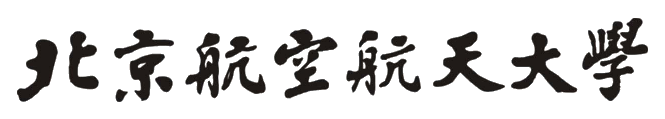
\includegraphics[width=8.8cm]{logo-buaa.eps}
\end{center}

\vspace{0.15cm}

\begin{center}

\includegraphics[width=12.8cm]{postdoc.png}
% 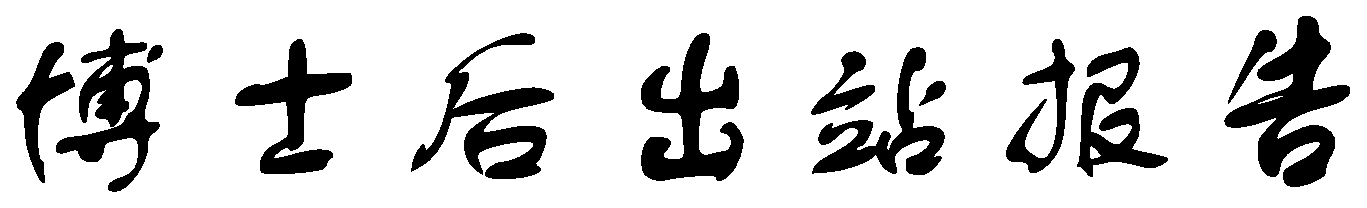
\includegraphics[width=12.8cm]{postdoc1.eps}
\end{center}

\vspace{0.15cm}

\begin{center}
{\erhao\song{\bf 联邦学习中模型个性化算法研究}}
\end{center}

\vspace{0.05cm}

\begin{spacing}{2}
\begin{center}{\erhao\bf
Study of Model Personalization Methods in Federated Learning}
\end{center}
\end{spacing}

\vspace{0.05cm}

\begin{center}
{\xiaoerhao\song\boldmath\bf 文豪}
\end{center}

\vspace{0.15cm}

\begin{tabbing} %tabbing 列表

\hspace*{3cm} \= \hspace{2.6cm} \= \kill
% \= in tabbing environment, sets a tab stop
% \kill in a\tabbing environment, deletes previous line so tabs can be set without outputting text.
% \> in tabbing environment is a forward tab.
% 这次的居中 用的 \centering ,注意三次的区别。
\>{\song\sihao\textbf {研\hspace{0.3cm}究\hspace{0.3cm}方\hspace{0.3cm}向\hspace{0.3cm} :}} \>
{\centering\song\sihao\textbf{~~~~~~~~~~联邦学习~~~~~~~~~~~~~}}\\
% 总长3.4cm
\\
\>{\song\sihao\textbf {合\hspace{0.3cm}作\hspace{0.3cm}导\hspace{0.3cm}师\hspace{0.3cm} :}}\>
{\centering\song\sihao\textbf{~~~~~~~~~~韩德仁~~~~教授~~~~~~~~~~~}} \\
\\
\>{\song\sihao\textbf {工作完成日期 \ \ :}}\> {\centering\song\sihao\textbf{~~~~~~~~~~2021年3月 --- 2023年6月~~~~~~~~~~}}\\
\\
\>{\song\sihao\textbf {报告提交日期 \ \ :}}\> {\centering\song\sihao\textbf{~~~~~~~~~~2023 年6月~~~~~~~~~~}} \\

\end{tabbing}

\vspace{0.1cm}
\begin{center}
{\song\boldmath \sihao ~2023~年~6~ 月}
\end{center}


\pagenumbering{Roman}

% \newcommand{\upcite}[1]{\textsuperscript{\textsuperscript{\cite{#1}}}}

\baselineskip 18.8pt

\chapter*{摘~~~要}
\headheight=15.24pt%5mm
\markboth{摘~~~要}{摘~~~要}
\addcontentsline{toc}{chapter}{{{\hei 摘~要}}\numberline ~}
\addcontentsline{toe}{chapter}{{{Abstract in Chinese}}\numberline ~}
\pagenumbering{Roman}\setcounter{page}{1}%非常重要的命令

待写


\par
\bigskip

{\song \textbf{关键词}: 待写}

\newpage
~~~\vspace{1em}
\thispagestyle{empty}

\chapter*{{Abstract}}%\vskip1cm
 \headheight=15.24pt%5mm
\markboth{Abstract} {Abstract}
 \headheight=15.24pt%5mm
\addcontentsline{toc}{chapter}{{{\bf Abstract}}\numberline ~~~}
\addcontentsline{toe}{chapter}{{{\bf Abstract in English}}\numberline ~}
\pagenumbering{Roman}\setcounter{page}{2}

to write


\par
\bigskip

{\bf Key words:} to write

%\nopagebreak[4]
\newpage
~~~\vspace{1em}
\thispagestyle{empty}



%%\mbox{}\newpage
\chapter*{符~号~说~明}
\headheight=15.24pt%5mm
\addcontentsline{toc}{chapter}{\numberline {{\heiti 符~号~说~明}}~~~}
\addcontentsline{toe}{chapter}{{{\bf Notation}}\numberline~}
\markboth{符~号~说~明}{北京航空航天大学文豪博士后研究工作报告}
%%%%%%%%%%%%%%%%%%%%%%%%%%%%%%%%%%%%%%%%%%%%%%%%%%%%%%%%%5
这里给出本文常用的一些符号, 未包含其中的符号将在文中用到时具体说明.
\begin{equation*}
  \begin{array}{lll}
\mathbb{R}&\qquad\qquad\qquad\qquad\qquad&\text{实数集}\\
\mathbb{C}&&\text{复数集}\\
\mathbb{R}^{n} &&\text{实~$n$ 维列向量集} \\
\mathbb{C}^{n} &&\text{复~$n$ 维列向量集} \\
\mathbb{R}^{m\times n} && \text{实~$m\times n$ 矩阵的集合} \\
\mathbb{C}^{m\times n} && \text{复~$m\times n$ 矩阵的集合} \\
%\mathbf{0}&& \text{零向量或零矩阵}\\
%\nabla &&\text{梯度算子} \\
%\nabla \cdot  &&\text{散度算子} \\
%%\nabla \times  &&\text{旋度算子} \\
%\Delta  &&\text{拉普拉斯算子} \\
\mathrm{i}&&\text{虚单位}\\
\overline{\theta} && \text{复数~$\theta$~的共轭}\\
|\cdot| &&\text{实数的绝对值或复数的模}\\
I_n~\text{或}~I &&\text{($n$~阶)单位矩阵}\\
O_n~\text{或}~O &&\text{($n$~阶)零矩阵}\\
A^\mathrm{T} &&\text{矩阵~$A$~的转置矩阵}\\
A^* &&\text{矩阵~$A$~的共轭转置矩阵}\\
A^{-1}&&  \text{矩阵~$A$~的逆矩阵}\\
\sigma(A)&&\text{矩阵~$A$~的谱集}\\
\rho(A) &&\text{矩阵~$A$~的谱半径}\\
\nu(A) &&\text{矩阵~$A$~的拟谱半径}\\
%\lambda_{\min}(A)&&\text{矩阵~$A$~的最小特征值}\\
%\lambda_{\min}^+(A)&&\text{矩阵~$A$~的最小正特征值}\\
%\lambda_{\max}(A)&&\text{矩阵~$A$~的最大特征值}\\
\mathrm{rank}(A)&&\text{矩阵~$A$~的秩}\\
\mathrm{null}(A)&&\text{矩阵~$A$~的零空间}\\
\mathrm{range}(A)&&\text{矩阵~$A$~的值域}\\
\mathrm{index}(A)&&\text{矩阵~$A$~的指标}\\
%\mathrm{tr}(A)&&\text{矩阵~$A$~的迹}\\
A\otimes B&&\text{矩阵~$A$~和~$B$~的\,Kronecker\,积}\\
\|\cdot\|_2&&\text{向量或矩阵的~$2$-范数}\\
%\|\cdot\|_A$$ && \text{向量的~$A$-范数}\\
%\|\cdot\|_F&&\text{矩阵的\,Frobenius\,范数}\\
A\succ O&&\text{矩阵\,$A$\,为对称正定矩阵}\\
\mathrm{span}\{x_1,\cdots,x_n\}&&\text{向量~$x_1,\cdots,x_n$~张成的线性空间}
\end{array}
\end{equation*}
\nopagebreak[4]


\tableofcontents
\tableofengcontents
\mainmatter

%\mbox{}\newpage
\chapter{\hspace{-1mm}\bf 绪论及预备知识}
\label{chap1}
\addcontentsline{toe}{chapter}{{{\bf Chapter 1\ \
Introduction  and Preliminaries }}\numberline\,}
\markboth{第\,1\,章\ \
绪论及预备知识}{北京航空航天大学博士后研究工作报告}
%%%%%%%%%%%%%%%%%%%%%%%%%%%%%%%%%%%%%%%%%%%%%%%%%%%%%%%%%%%
\section{绪论}
\addcontentsline{toe}{section}{{1.1\ \ Introduction}\numberline\,}
\label{sec:introduction}

% almost finished

随着人工智能、大数据等技术的飞速发展,特别是物联网(Internet of Things, IoT)的快速普及,可用于机器学习研究的数据呈爆发式增长,其来源与分布的形式也越来越多样化。这种变化趋势给机器学习的研究与应用带来了前所未有的挑战,也提供了崭新的发展机遇。

传统上来说,机器学习的范式是将要研究的数据集中到一起,例如一个数据中心,进行建模方法、优化算法等方面的研究。然而随着上文提到的研究数据来源与分布的形式的多样化,将数据集中到一起面临越来越大的困难。举例来说,执行某一类任务的物联网设备往往数量庞大,数量级以百万乃至千万计,其产生的数据总量巨大。但是物联网设备的通信带宽往往不高,相互之间的通信,以及与数据中心之间的通信往往会有较高的延迟。在这种场景下,将感兴趣的数据集中到一起进行研究,是极其困难,成本非常高的。与此同时,随着人们的隐私保护意识越来越强,相关的法律法规,例如欧盟2018年正式生效的《General Data Protection Regulation》,越来越严格,收集用户的数据也越来越困难\citep{Albrecht_2016}。例如,用户的键盘输入数据可以用于训练输入自动补全的模型,提高用户输入效率\citep{fl_keyboard}。一般来说,通信带宽不是这类数据共享的瓶颈,但是基于隐私法律法规的限制,收集此类数据限制极大。还有一些类型的数据是具有高度机密性的数据,例如医疗、金融数据。相关的医疗机构之间或者金融机构之间往往不会进行数据共享。

在很多场景下,数据孤岛的效应比较突出:各个数据持有方持有的数据量严重不平衡,分布差异性大。如果各个数据持有方仅仅依赖各自拥有的本地数据进行模型训练,得到的机器学习模型往往是严重过拟合的,实际使用效果往往不佳。

因此,如何在尽可能地保证质量的前提下,高效率地进行分布式的机器学习模型的训练,这一问题的重要性越来越突出。因为场景的多样性,或者说数据分布的多样性,以及相应需求的多样性,一个普适的、能满足所有需求的分布式机器学习模型训练的范式是不存在的,很多时候必须有侧重地针对某一部分需求设计相应的分布式学习方法,例如侧重隐私性的差分隐私方法(Differential Privacy)\citep{Dwork_2008_DP}, 侧重模型训练效果的优化算法设计\citep{boyd2011distributed}等。这些问题还有很多亟待改进与完善,具有关阔的研究前景与巨大的应用价值。

\section{联邦学习的起源与发展}
\addcontentsline{toe}{section}{{1.2\ \ Origin and Development of Federal Learning}\numberline\,}
\label{sec:fl_origin}

待写

%\mbox{}\newpage
\chapter{\hspace{-1mm}\bf 待写}
\label{chap2}
\addcontentsline{toe}{chapter}{{{\bf Chapter 2\ \
To write }}\numberline\,}
\markboth{第\,2\,章\ \
待写}{北京航空航天大学博士后研究工作报告}
%%%%%%%%%%%%%%%%%%%%%%%%%%%%%%%%%%%%%%%%%%%%%%%%%%%%%%%%%%%
\section{待写}
\addcontentsline{toe}{section}{{2.1\ \ To write}\numberline\,}

待写

%\mbox{}\newpage
\chapter{\hspace{-1mm}\bf 待写}
\label{chap3}
\addcontentsline{toe}{chapter}{{{\bf Chapter 3\ \
To write }}\numberline\,}
\markboth{第\,3\,章\ \
待写}{北京航空航天大学博士后研究工作报告}

%%%%%%%%%%%%%%%%%%%%%%%%%%%%%%%%%%%%%%%%%%%%%%%%%%%%%%%%%%%

\section{联邦学习中的模型个性化问题}
\addcontentsline{toe}{section}{{3.1\ \ To write}\numberline\,}

待写。。。。

\section{个性化联邦学习中的典型算法}
\addcontentsline{toe}{section}{{3.2\ \ To write}\numberline\,}

待写。。。。

\section{个性化联邦学习中的算子分裂算法}
\addcontentsline{toe}{section}{{3.3\ \ To write}\numberline\,}

待写。。。。

%\mbox{}\newpage
\chapter{\hspace{-1mm}\bf 待写}
\label{chap4}
\addcontentsline{toe}{chapter}{{{\bf Chapter 4\ \
To write }}\numberline\,}
\markboth{第\,4\,章\ \
待写}{北京航空航天大学博士后研究工作报告}

%%%%%%%%%%%%%%%%%%%%%%%%%%%%%%%%%%%%%%%%%%%%%%%%%%%%%%%%%%%

待写。。。。


\printbibliography[title=参考文献]

\backmatter
\chapter*{博士后在站期间的主要成果}
\addcontentsline{toc}{chapter}{{博士后在站期间的主要成果}\numberline~~~}
\addcontentsline{toe}{chapter}{{Main achievements during the postdoctoral program}\numberline ~~~}
\markboth{博士后在站期间的主要成果}{博士后在站期间的主要成果}\headheight=15.24pt%5mm

\noindent{\larger \heiti 基金项目:}

\begin{itemize}
    \item 面向脊柱穿刺消融手术的多模态图像导航关键算法研究,数学天元基金项目/数学天元基金/数学与医疗健康交叉重点专项,参与,起止时间:2022/01 -- 2023/12。
    \item 数字电路物理设计自动化中关键数学问题研究,国家重点研发计划,参与,起止时间:2022/05 -- 2025/04。
\end{itemize}

\noindent{\larger \heiti 科研论文:}

\begin{enumerate}
    \item WEN H, KANG J. Hybrid Arrhythmia Detection on Varying-Dimensional Electrocardiography: Combining Deep Neural Networks and Clinical Rules[C]//2021 Computing in Cardiology (CinC): vol. 48. Institute of Electrical and Electronics Engineers (IEEE), 2021. DOI: 10.23919/cinc53138.2021.9662801.
    \item KANG J, WEN H. A Study on Several Critical Problems on Arrhythmia Detection using Varying-Dimensional Electrocardiography[J]. Physiological Measurement, 2022, 43(6): 064007. DOI: 10.1088/1361-6579/ac6aa3.
    \item WEN H, KANG J. A Novel Deep Learning Package for Electrocardiography Research[J]. Physiological Measurement, 2022, 43(11): 115006. DOI: 10.1088/1361-6579/ac9451.
    \item WEN H, KANG J. A Comparative Study on Neural Networks for Paroxysmal Atrial Fibrillation Events Detection from Electrocardiography[J]. Journal of Electrocardiology, 2022, 75: 19-27. DOI: 10.1016/j.jelectrocard.2022.10.002.
    \item GU E, CHEN Y, WEN H, CAI X, HAN D. Novel Clustered Federated Learning Based on Local Loss. 2023. Submitted.
\end{enumerate}

% \patchcmd{\thebibliography}{\section*}{\chapter*}{}{}

% \begin{refsection}[publications.bib]
% \nocite{wen_cinc2021, Kang_2022_cinc2021_iop, torch_ecg_paper, Wen_cpsc2021, wen_cinc2022}
% \printbibliography[title={\heiti 科研论文}]
% \end{refsection}


\chapter*{致~~~谢}\vskip1cm
\addcontentsline{toc}{chapter}{{致谢}\numberline ~~~}
\addcontentsline{toe}{chapter}{{Acknowledgement}\numberline ~~~}
\markboth{致~~~谢}{北京航空航天大学博士后研究工作报告}
\vspace{-1.0cm}

% finished

首先,我衷心感谢我合作导师韩德仁教授,感谢他将联邦学习这一国际前沿的研究领域介绍给我,以他的博学多识以及敏锐的直觉,给我指引研究的方向,对相关的难点问题对我进行悉心的指导,使我受益匪浅。

我要感谢北京航空航天大学数学科学学院统计与运筹系以及计算科学系的老师以及同学们:崔春风、谢家新、邓钊、于冬梅、黄博、靳正芬、陈彩荣、路宁、顾恩东、屈云飞、陈鑫、陈永鑫、王青松、胡乐宇、苏宴生、刘锐、苌远等,以及南京师范大学的蔡邢菊教授,协助我组织联邦学习讨论班,积极参与问题的讨论,在我的研究过程中给了我很多有益的建议,对我的帮助极大。

我要感谢北京航空航天大学数学科学学院的行政机关的老师们:齐丹、陆筱、赵丽君、鲁琛、曹安妮、李田田、徐田梅,他们出色而专业的工作,保障了我科研工作的顺利进行。

我还要感谢我的父母,我的妻子,我的岳母还有我的女儿,给我鼓励与支持,让我没有后顾之忧,让我能够全情投入于博士后课题的研究。

\vspace{-2cm}
\textit{ \vskip 1in \centerline{{\mbox{}\hskip 13cm}文豪}
\vskip 0in
\centerline{{\mbox{}\hskip 12.3cm}2023\,年\,6\,月}
}


\end{document}
